\chapter{Startup Design Lab}

Lo \emph{Startup Design Lab} è il progetto di questo corso nel quale si vedrà
come portare alla luce le idee per una startup, partendo dalla genesi, passando
per definizione di un business model efficace per arrivare alla presentazione
del progetto.

\section{Passi per creare una startup}

\begin{itemize}
 \item[Tema] È importante scegliere il tema e formare un team
 \item[Analisi] Fare un'analisi di mercato, individuare i competitor e le
tecnologie
 \item[Idee] Dal brainstorming alla generazione dell'idea
 \item[Selezione] In cui si effettua \textit{Kill\&Thrill} e si fa una draft
del business model
 \item[Business Model] Si esegue il design e l'analisi SWOT
 \item[BM Finale] Che include le \textit{personae}, il BM in
dettaglio e il posizionamento nel mercato
 \item[Finance] Si eseguono Business plan, Breakeven e si pensa al ROI
 \item[Presentazione] \textit{Pitch} di presentazione della start-up
\end{itemize}

I gruppi variano dalle 3 alle 4 persone, massimo 5. Questa quantità garantisce
una buona variabilità all'interno del gruppo stesso e permettendo a tutti i
membri di esprimersi.

\section{Dal tema all'idea}

\subsection{Tema}
Per \textbf{tema} della startup si intende l'argomento generico del progetto,
ma non in dettaglio: si arriva a identificare qual è l'argomento che suscita
curiosità e attorno al quale si vuole generare l'idea di startup. In caso non
ci siano delle idee, è consigliato seguire questi tre passaggi:
\begin{enumerate}
 \item Scelta dell'elemento tecnologico della startup su cui far leva per la
 scalabilità e per gli altri argomenti che sono stati discussi a lezione e nei
 capitoli precedenti;
 \item Scelta del tema a cui applicare la tecnologia. È possibile anche
 prendere una tecnologia già esistente ed applicarla ad un altro contesto;
 \item Scegliere a chi è rivolta tale tecnologia.
\end{enumerate}

\subsection{Analisi}
Una volta trovato il tema, si passa alla fase di \textbf{analisi} di quanto
definito al passo precedente. In questo momento è importante studiare la
mortalità delle startup nello stesso campo scelto: se essa è troppo alta
infatti significa che è molto probabile incorrere in un fallimento, o è
necessario analizzare in precisione qual è stata la causa del loro
insuccesso.

\subsubsection{Competitor}
In generale, è sempre utile analizzare i \textbf{competitor}, vedere se sono
partiti da startup e/o da chi sono finanziati, e verificare se l'ambito in cui
ci si sta per buttare è già affollato o se c'è poca gente. Anche la dimensione
delle aziende conta: avere come competitor poche piccole startup è molto
diverso dal confrontarsi con poche ma grandi aziende.

\subsubsection{Tecnologie}
Una volta analizzati i competitor è anche importante studiare la
\textbf{tecnologia} che si andrà a usare, le sue caratteristiche ma anche i
suoi costi.

\subsubsection{Trend di settore}
Successivamente è importante andare studiare e cercare di prevedere come il
mercato si potrà evolvere negli anni a venire in quel determinato settore.
Per esempio, aprire una nuova tipologia di distributore di benzina è un'idea a
breve termine, in quanto nel futuro le energie non rinnovabili andranno ad
esaurirsi. Al contrario, investire in mercati nei quali è possibile richiedere
fondi (allo stato o alla comunità europea) può essere una buona mossa per
avere un budget iniziale e convincere anche eventuali investitori ad
investire nella realtà che si sta tentando di creare. Un esempio è il campo
delle energie rinnovabili.

Il grafico di posizionamento permette di capire eventuali competitor nel
mercato (i \textbf{trend}), per identificare eventuali fasce di mercato
``libere''.
In tale grafico si definisce un piano con le ascisse e le ordinate che
rappresentano delle caratteristiche che si ritengono significative e
successivamente si inseriscono i competitor o i prodotti
differenti dal nostro. La scelta degli assi è difficoltosa: oltre che
rilevanti, tali caratteristiche dovrebbero essere anche oggettive (un cattivo
esempio potrebbe essere la qualità: è di sicuro un'ottima caratteristica di un
prodotto ma la sua valutazione è del tutto soggettiva). Nel caso in cui gli
assi si rivelino non significativi si possono avere tutti i valori distribuiti
nello stesso quadrante, in soli due quadranti o, nel caso in cui i valori degli
assi siano correlati, distribuiti a formare una diagonale. Gli elementi da
inserire in questo grafico sono i competitor scovati nelle fasi precedenti.

\begin{figure}[t]
  \centering
  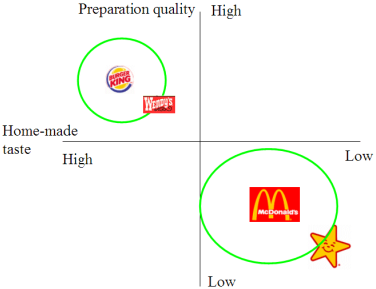
\includegraphics[scale=0.7]{competitor_analysis}
  \caption{Un esempio di un grafico con i competitor}
  \label{fig:dsl:ca}
\end{figure}


I social network sono in grado di fare un'analisi di mercato molto precisa,
grazie alla profilazione.

Il posizionamento di un brand è deciso dalle strategie che compie e dal mercato
stesso. Quando le aspettative del brand non sono le stesse del mercato
l'azienda esegue quello che è definito come un riposizionamento di mercato,
ovvero si cambia la percezione degli utenti che hanno sull'azienda stessa. La
difficoltà in tutto ciò è cambiare l'immagine che tutti gli utenti hanno, ed è
un'operazione onerosa e lenta.
